%% LaTeX Beamer presentation template (requires beamer package)
%% see http://latex-beamer.sourceforge.net/
%% idea contributed by H. Turgut Uyar
%% template based on a template by Till Tantau
%% this template is still evolving - it might differ in future releases!

%
% This document content was realized for the Marcusevans presentation
% on June 17th 2010
%
% Authors: ekeller
%



%\documentclass[handout]{beamer}
\documentclass{beamer}


\mode<presentation>
{
\usetheme{Warsaw}
\setbeamercovered{transparent}
% added the frame numbers 2010-05-28 by ekeller
\setbeamertemplate{footline}
{%
\begin{beamercolorbox}[wd=0.5\textwidth,ht=3ex,dp=1.5ex,leftskip=.5cm,rightskip=.5cm]{author in head/foot}%
\usebeamerfont{author in head/foot}%
\insertframenumber/\inserttotalframenumber\hfill\insertshortauthor%
\end{beamercolorbox}%
\vspace*{-4.5ex}\hspace*{0.5\textwidth}%
\begin{beamercolorbox}[wd=0.5\textwidth,ht=3ex,dp=1.5ex,left,leftskip=.5cm]{title in head/foot}%
\usebeamerfont{title in head/foot}%
\insertshorttitle%
\end{beamercolorbox}%
} 
}

\usepackage[english]{babel}
\usepackage[latin1]{inputenc}
% for image animation purpose
\usepackage{xmpmulti}

% font definitions, try \usepackage{ae} instead of the following
% three lines if you don't like this look
\usepackage{mathptmx}
\usepackage[scaled=.90]{helvet}
\usepackage{courier}


\usepackage[T1]{fontenc}


\title[Industrialisierung Embedded Software Engineering: CI]{Continuous
Integration}

%\subtitle{at HAMILTON-Medical AG}

% - Use the \inst{?} command only if the authors have different
%   affiliation.
%\author{F.~Author\inst{1} \and S.~Another\inst{2}}
\author{Eric Keller}

% - Use the \inst command only if there are several affiliations.
% - Keep it simple, no one is interested in your street address.
\institute[HAMILTON-Medical AG]
{
HAMILTON-Medical AG\\
}

\date{2010-06-17 / Industrialisierung Embedded Software Engineering}

% This is only inserted into the PDF information catalog. Can be left
% out.
\subject{Talks}



% If you have a file called "university-logo-filename.xxx", where xxx
% is a graphic format that can be processed by latex or pdflatex,
% resp., then you can add a logo as follows:

\pgfdeclareimage[height=0.5cm]{hamilton-logo}{../img/hamilton-logo.jpg}
\logo{\pgfuseimage{hamilton-logo}}


% Delete this, if you do not want the table of contents to pop up at
% the beginning of each subsection:
%\AtBeginSubsection[]
%{
%\begin{frame}<beamer>
%\frametitle{Outline}
%\tableofcontents[currentsection,currentsubsection]
%\end{frame}
%}

% If you wish to uncover everything in a step-wise fashion, uncomment
% the following command:

%\beamerdefaultoverlayspecification{<+->}

\begin{document}

% this braket defines that the background template should only be used for this
% frame
{
% set the hamilton.jpg as background image
\usebackgroundtemplate{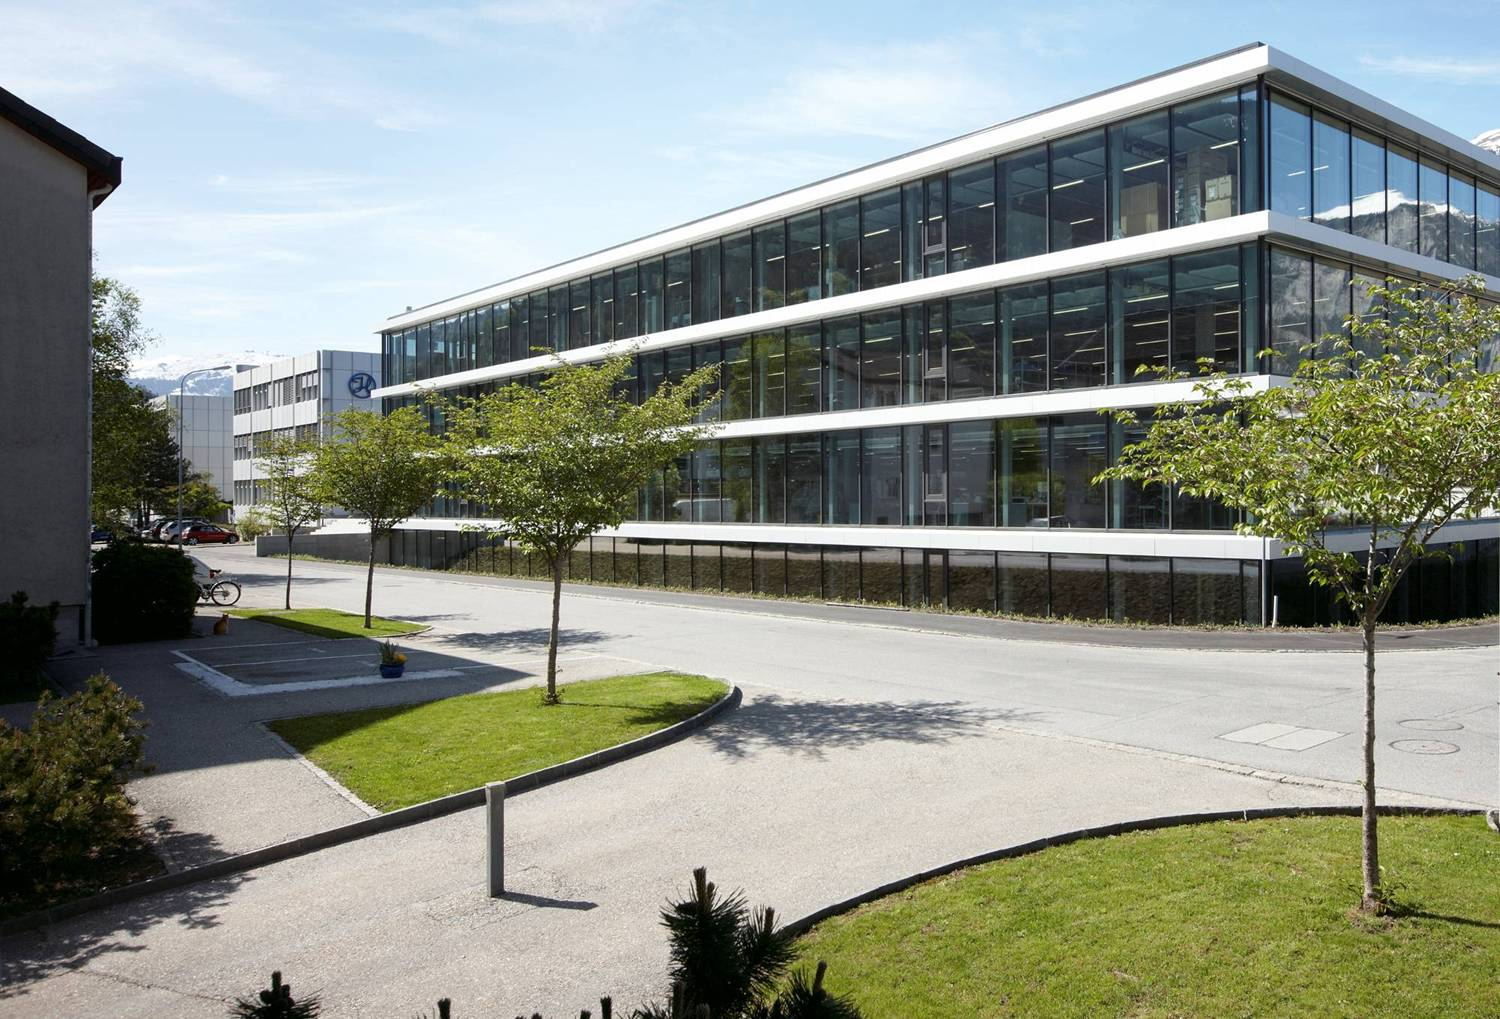
\includegraphics[width=\paperwidth,height=\paperheight]{../img/hamilton.jpg}}
\begin{frame}[shadow=false]
\titlepage
\end{frame}
}
% goal and policy
%\section*{Presentation goals and policy}
\begin{frame}
\frametitle{Goals}
Goals:
\begin{itemize}
  \item<1-> Give an overview of what can be achieved with Continuous Integration
  (CI)
  \item<2-> Share knowledge and ideas
\end{itemize}
\onslide<3->{
\begin{block}{Presentation rule}
   \alert{Please note your question and keep them warm for the end of the
   presentation}
 \end{block}
}
\end{frame}

\begin{frame}
\frametitle{Outline}
\tableofcontents[pausesections]
% You might wish to add the option [pausesections]
\end{frame}

%% frame pattern
%\begin{frame}
%\frametitle{}
%\framesubtitle{Subtitles are optional}
%\end{frame}

\section{Introduction}

\subsection[About Hamilton-Medical]{About Hamilton-Medical}
\begin{frame}
\frametitle{Activities and organisation}
\begin{columns} 
  	\column{.5\textwidth}
\onslide<1->{
    \begin{block}{Platform G}
      \begin{center}
		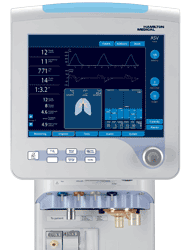
\includegraphics[height=2cm]{../img/G5.png}
      \end{center}
    \end{block}
}
\onslide<2->{
    \begin{block}{Accessories}
      \begin{center}
		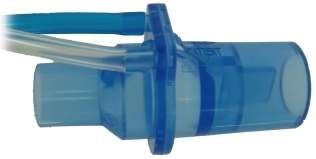
\includegraphics[height=2cm]{../img/flowsensor.png}
      \end{center}
    \end{block}
}
\column{.5\textwidth}
\onslide<3->{
    \begin{block}{Platform C}
      \begin{center}
		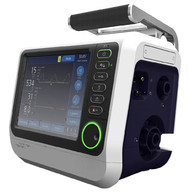
\includegraphics[height=2cm]{../img/C1.png}
		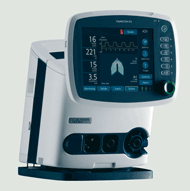
\includegraphics[height=2cm]{../img/C2.png}
      \end{center}
    \end{block}
}
\end{columns}

\end{frame}

\subsection[Developer environment]{Developer environment}
\begin{frame}{Host development tools}
The Platform C Projects are developed on Microsoft Windows Host, using the
following software and hardware:
\begin{columns}
	\column{.5\textwidth}
	\begin{block}{Software Development}
	\begin{itemize}
		\item<1-> IBM Rational Rhapsody
  		\item<2-> WindRiver Workbench (eclipse) 
  		\item<3-> IPL Cantata++
    \end{itemize}
    \end{block}

	\begin{block}{Other used tools}
	\begin{itemize}
      \item<4-> shell, perl, scripting
      \item<5-> PVCS version manager
      \item<6-> ScrumWorks 
    \end{itemize}
    \end{block}

	\column{.5\textwidth}
	\begin{block}{Target Development}
	\begin{itemize}
      \item<7->WindRiver VxWorks 6.4
  	  \item<8-> Power PC MPC5200 B
    \end{itemize}
    \end{block}
\end{columns}
\end{frame}

\begin{frame}
\frametitle{Continuous Integration key notes}
\begin{itemize}
  \item<1-> CI is a software development practice where software parts are
  integrated frequently
  \item<2-> Each integration step is verified by an automated process
  \item<3-> Find problems as soon as possible
  \item<4-> Make it easy for anyone to get the latest executable
  \item<5-> CI is all about communication
\end{itemize}
\end{frame}

\section[Automated build and test]{Automated build and test}
\subsection[Technical notes]{Technical notes}

\begin{frame}
\frametitle{Development tools interaction}
\setbeamercovered{invisible}
\centering
\multiinclude[format=png,graphics={scale=0.3}]{../img/toolintegration}
\end{frame}

\subsection[Good practices]{Good practices}
\begin{frame}
\frametitle{Good practices}
\begin{itemize}
  \item<1-> Everyone in the team integrates frequently (daily)\cite{Fowler06}
  \item<2-> Self-testing code when writing code, also write test for
  that code\cite{Duvall07}
  \item<3-> Imperfect test running frequently are better than perfect test that
  are never written at all\cite{Duvall07}
  \item<4-> Not allowed to fix before corresponding test exists
  \item<5-> Never check-in broken code\cite{Berczuk03} 
  \item<6-> If it happens, fix the broken build as quick as possible 
\end{itemize}
\end{frame}


\subsection[Prerequisites]{Prerequisites}

\begin{frame}
\frametitle{Prerequisites}

\begin{itemize}
  \item<1-> A decent Source Code Management system (SCM)\cite{Berczuk03}
  \item<2-> Everything you need to fullfil a software build should be checked in
  the repository\cite{Berczuk03} (scripts, 3rd party libraries,\ldots)
  \item<3-> Automated build sequence
  \item<4-> Automated test builds and run
  \item<5-> Automated documentation generation
  \item<6-> Automated deployment (software package)  
\end{itemize}

\onslide<7->{
\begin{block}{Note}
   \alert{in this case ``automated'' means, one command to do everything}
 \end{block}
}
\end{frame}

\section[Automated deployment]{Automated deployment}
\subsection[Notifications and list of changes]{Notifications and list of
changes}
\begin{frame}
\frametitle{Notifications and list of changes}
\onslide<1->
{
\begin{block}{Software engineers}
   \begin{itemize}
     \item<1-> See in Real time, the state of the CI builds
     \item<2-> Get notified, when a build fails/succeed
     \item<3-> Get a complete change log and diff over the complete
     project between each commit
   \end{itemize}
 \end{block}
}
\onslide<4->
{
\begin{block}{QA, PM, Documentation}
   \begin{itemize}
     \item<4-> Get notified when a release build succeeds
     \item<5-> Get the detailed change log between two builds, list new
     features, fixes, between each commit.
   \end{itemize}
 \end{block}
}

\end{frame}

\subsection[Get the latest versions]{Get the latest versions}
\begin{frame}
\frametitle{Get the latest versions}

\begin{itemize}
  \item<1-> Everyone involved in the project should be able to get
  and run the latest software version
  \item<2-> Get the latest software version anytime for demonstration, testing,
  or just to notice the change of this week
  \item<3-> Easy to find, download, run (Web client) 
\end{itemize}

\end{frame}


\subsection[Get feedbacks]{Get feedbacks}
\begin{frame}
\frametitle{Get feedbacks}

\begin{itemize}
  \item Users are able to tag/comment the build, depending on its stability,
  the number of failing tests, test coverage, \ldots
  \item Frequent software deployment allows to get new features more rapidly to
  get more rapid feedback\cite{Fowler06} from end users
\end{itemize}

\end{frame}


\section*{Overview of Hamilton process}
\begin{frame}
\frametitle<presentation>{Overview of Hamilton process}

\setbeamercovered{invisible}
\centering
\multiinclude[format=png,graphics={scale=0.3}]{../img/continuous_integration}

\end{frame}

\section[Benefits and optimisations]{Benefits and optimisations}
\subsection[Benefits]{Benefits}
\begin{frame}
\frametitle{Benefits}
\begin{itemize}
	\item<1-> Reducing risk, increase software quality 
    \item<2-> short integration time 
    \item<3-> Bugs are detected quickly, depending on how good the test suite
    is\cite{Duvall07}
    \item<4-> Easier to fix bugs (diff debug)
    \item<5-> More frequent demonstration of new features, more collaboration
    between developers, PM, QA, \ldots
    \item<6-> More frequent releases
    \item<7-> Frequent customer feedback, improve customer requirement
    fullfility
\end{itemize}
\end{frame}

\subsection[Optimisations]{Optimisations}

\begin{frame}
\frametitle{Optimisations}
\begin{itemize}
	\item<1-> Staged build, several type of builds\cite{Fowler06}
		\begin{itemize}
          \item<2-> Commit build (triggered by repository) has to be done
          quickly
          \item<3-> Secondary builds (when the commit build is successful) build
          and run tests
          \item<4-> Third builds, generate test documentation, summaries and
          provide build metrics\cite{Duvall07}
        \end{itemize}
    \item<5-> Keep the commit build fast\cite{Duvall07} (~10-20 min.)
    \begin{itemize}
      \item perform a clean build
      \item use all your CPU to build faster
      \item distribute your compilation over a computer farm\cite{Pool09}
      \item eventually perform incremental builds instead of clean build
    \end{itemize}
    \item<6-> Prevent checking in broken code, by performing a private
    build\cite{Duvall07}
    \item<7-> Partially automate integration/system tests (smoke
    test)\cite{Berczuk03}
\end{itemize}
\end{frame}

\begin{frame}{Further lectures}
\begin{thebibliography}{8}

\bibitem{Fowler06}[Fowler, 2006]
	Martin Fowler
	\newblock Continuous Integration
	\url{http://martinfowler.com/articles/continuousIntegration.html}
	\newblock this website provides several key steps to setup CI

\bibitem{Duvall07}[Duvall, 2007]
	Paul M. Duvall
	\newblock Professional Continuous Integration Improving Software Quality and
	Reducing Risk
	\newblock this book contains all the details about continuous integration

\bibitem{Berczuk03}[Berczuk, 2003]
	Stephen P. Berczuk
	\newblock Software Configuration Management Patterns
	\newblock more details about the integration builds and the Private builds
	
\bibitem{Pool09}[Pool, 2009]
	Martin Pool
	\newblock distcc: a fast, free distributed C/C++ compiler
	\url{http://code.google.com/p/distcc/}
	\newblock Learn more about efficiently distribute your compilation for gaining
	time

\end{thebibliography}
\end{frame}

\begin{frame}
\frametitle{Questions}
\end{frame}

\end{document}
